
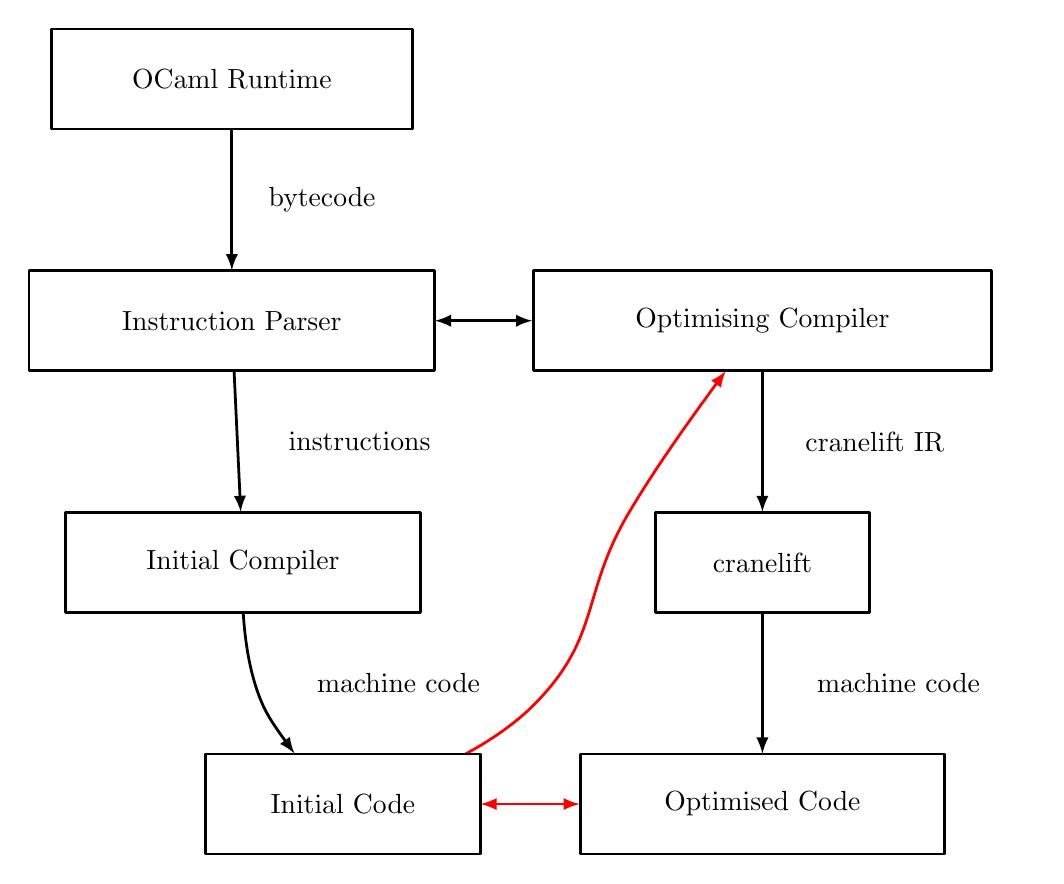
\begin{tikzpicture}[>=latex,line join=bevel,]
  \pgfsetlinewidth{1bp}
%%
\begin{scope}
  \pgfsetstrokecolor{black}
  \definecolor{strokecol}{rgb}{1.0,1.0,1.0};
  \pgfsetstrokecolor{strokecol}
  \definecolor{fillcol}{rgb}{1.0,1.0,1.0};
  \pgfsetfillcolor{fillcol}
  \filldraw (0.0bp,0.0bp) -- (0.0bp,297.0bp) -- (362.0bp,297.0bp) -- (362.0bp,0.0bp) -- cycle;
\end{scope}
\begin{scope}
  \pgfsetstrokecolor{black}
  \definecolor{strokecol}{rgb}{1.0,1.0,1.0};
  \pgfsetstrokecolor{strokecol}
  \definecolor{fillcol}{rgb}{1.0,1.0,1.0};
  \pgfsetfillcolor{fillcol}
  \filldraw (0.0bp,0.0bp) -- (0.0bp,297.0bp) -- (362.0bp,297.0bp) -- (362.0bp,0.0bp) -- cycle;
\end{scope}
\begin{scope}
  \pgfsetstrokecolor{black}
  \definecolor{strokecol}{rgb}{1.0,1.0,1.0};
  \pgfsetstrokecolor{strokecol}
  \definecolor{fillcol}{rgb}{1.0,1.0,1.0};
  \pgfsetfillcolor{fillcol}
  \filldraw (0.0bp,0.0bp) -- (0.0bp,297.0bp) -- (362.0bp,297.0bp) -- (362.0bp,0.0bp) -- cycle;
\end{scope}
  \pgfsetcolor{black}
  % Edge: ocaml_runtime -> instruction_parser
  \draw [->] (73.0bp,260.8bp) .. controls (73.0bp,249.16bp) and (73.0bp,233.55bp)  .. (73.0bp,210.18bp);
  \definecolor{strokecol}{rgb}{0.0,0.0,0.0};
  \pgfsetstrokecolor{strokecol}
  \draw (105.5bp,235.5bp) node {bytecode};
  % Edge: instruction_parser -> optimising_compiler
  \draw [<->] (146.12bp,192.0bp) .. controls (161.16bp,192.0bp) and (166.08bp,192.0bp)  .. (181.11bp,192.0bp);
  % Edge: instruction_parser -> initial_compiler
  \draw [->] (73.809bp,173.8bp) .. controls (74.357bp,162.16bp) and (75.092bp,146.55bp)  .. (76.192bp,123.18bp);
  \draw (119.0bp,148.5bp) node {instructions};
  % Edge: optimising_compiler -> cranelift
  \draw [->] (264.0bp,173.8bp) .. controls (264.0bp,162.16bp) and (264.0bp,146.55bp)  .. (264.0bp,123.18bp);
  \draw (304.5bp,148.5bp) node {cranelift IR};
  % Edge: cranelift -> optimised_code
  \draw [->] (264.0bp,86.799bp) .. controls (264.0bp,75.163bp) and (264.0bp,59.548bp)  .. (264.0bp,36.175bp);
  \draw (313.0bp,61.5bp) node {machine code};
  % Edge: initial_compiler -> compiled_code
  \draw [->] (77.103bp,86.699bp) .. controls (77.721bp,76.765bp) and (79.471bp,64.265bp)  .. (84.0bp,54.0bp) .. controls (85.445bp,50.724bp) and (87.289bp,47.51bp)  .. (95.546bp,36.228bp);
  \draw (133.0bp,61.5bp) node {machine code};
  % Edge: compiled_code -> optimising_compiler
  \pgfsetcolor{red}
  \draw [->] (157.08bp,36.003bp) .. controls (166.06bp,40.865bp) and (174.92bp,46.835bp)  .. (182.0bp,54.0bp) .. controls (206.03bp,78.314bp) and (198.53bp,93.611bp)  .. (216.0bp,123.0bp) .. controls (224.7bp,137.63bp) and (235.56bp,153.2bp)  .. (250.79bp,173.89bp);
  % Edge: compiled_code -> optimised_code
  \draw [<->] (162.55bp,18.0bp) .. controls (177.79bp,18.0bp) and (182.99bp,18.0bp)  .. (198.21bp,18.0bp);
  % Node: instruction_parser
\begin{scope}
  \definecolor{strokecol}{rgb}{0.0,0.0,0.0};
  \pgfsetstrokecolor{strokecol}
  \draw (146.0bp,210.0bp) -- (0.0bp,210.0bp) -- (0.0bp,174.0bp) -- (146.0bp,174.0bp) -- cycle;
  \draw (73.0bp,192.0bp) node {Instruction Parser};
\end{scope}
  % Node: optimising_compiler
\begin{scope}
  \definecolor{strokecol}{rgb}{0.0,0.0,0.0};
  \pgfsetstrokecolor{strokecol}
  \draw (346.5bp,210.0bp) -- (181.5bp,210.0bp) -- (181.5bp,174.0bp) -- (346.5bp,174.0bp) -- cycle;
  \draw (264.0bp,192.0bp) node {Optimising Compiler};
\end{scope}
  % Node: cranelift
\begin{scope}
  \definecolor{strokecol}{rgb}{0.0,0.0,0.0};
  \pgfsetstrokecolor{strokecol}
  \draw (302.5bp,123.0bp) -- (225.5bp,123.0bp) -- (225.5bp,87.0bp) -- (302.5bp,87.0bp) -- cycle;
  \draw (264.0bp,105.0bp) node {cranelift};
\end{scope}
  % Node: initial_compiler
\begin{scope}
  \definecolor{strokecol}{rgb}{0.0,0.0,0.0};
  \pgfsetstrokecolor{strokecol}
  \draw (141.0bp,123.0bp) -- (13.0bp,123.0bp) -- (13.0bp,87.0bp) -- (141.0bp,87.0bp) -- cycle;
  \draw (77.0bp,105.0bp) node {Initial Compiler};
\end{scope}
  % Node: compiled_code
\begin{scope}
  \definecolor{strokecol}{rgb}{0.0,0.0,0.0};
  \pgfsetstrokecolor{strokecol}
  \draw (162.5bp,36.0bp) -- (63.5bp,36.0bp) -- (63.5bp,0.0bp) -- (162.5bp,0.0bp) -- cycle;
  \draw (113.0bp,18.0bp) node {Initial Code};
\end{scope}
  % Node: optimised_code
\begin{scope}
  \definecolor{strokecol}{rgb}{0.0,0.0,0.0};
  \pgfsetstrokecolor{strokecol}
  \draw (329.5bp,36.0bp) -- (198.5bp,36.0bp) -- (198.5bp,0.0bp) -- (329.5bp,0.0bp) -- cycle;
  \draw (264.0bp,18.0bp) node {Optimised Code};
\end{scope}
  % Node: ocaml_runtime
\begin{scope}
  \definecolor{strokecol}{rgb}{0.0,0.0,0.0};
  \pgfsetstrokecolor{strokecol}
  \draw (138.0bp,297.0bp) -- (8.0bp,297.0bp) -- (8.0bp,261.0bp) -- (138.0bp,261.0bp) -- cycle;
  \draw (73.0bp,279.0bp) node {OCaml Runtime};
\end{scope}
%
\end{tikzpicture}

